\documentclass[11pt,a4paper]{article}
\usepackage[utf8]{inputenc}
\usepackage[german]{babel}
\usepackage{amsmath}
\usepackage{amsfonts}
\usepackage{subfig}
\usepackage{amssymb}
\usepackage{siunitx,physics}
\usepackage{mathtools}
\usepackage{graphicx}
%\usepackage{Here}
\usepackage[version=4]{mhchem}
\usepackage{url}
\usepackage{setspace}
\usepackage[left=2.5cm,right=2.5cm,top=2.5cm,bottom=2cm]{geometry}
[biblography=totocnumbered]
\usepackage{fancyhdr}
\usepackage{scrextend}
\usepackage{hyperref}
\pagenumbering{gobble}

\makeatletter
\newcommand\bigcdot{\mathpalette\bigcdot@{.5}}
\newcommand\bigcdot@[2]{\mathbin{\vcenter{\hbox{\scalebox{#2}{$\m@th#1\bullet$}}}}}
\makeatother

\makeatletter
%\renewcommand*\bib@heading{%
%  \subsection*{}%
%  \@mkboth{\refname}{\refname}}
%\makeatother
\numberwithin{equation}{section}
\numberwithin{figure}{section}

\renewcommand{\labelitemii}{\labelitemfont$\vartriangleright$}
\begin{document}\\
\begin{addmargin}[25pt]{0pt}
Man muss die freie Enthalpie für verschiedene Temperaturen, wie in Abbildung \ref{fig:Mischungsenthalpie_Phasendiagramm}, gegen die Zusammensetzung auftragen. Sollte die freie Enthalpie für alle Zusammensetzungen für eine Phase kleiner sein, dann befindet man sich im Einphasengebiet dieser Phase. Das Zweiphasengebiet erkennt man daran, dass sich die freien Enthalpien bei diesen schneiden, in Abbildung \ref{fig:Mischungsenthalpie_Phasendiagramm} ist das bei $T_3$ und $T_4$ der Fall. In diesem Fall muss man noch die eine Tangente finden, welche sowohl für die feste als auch für die flüssige Phasen eine Tangente ist. Die Schnittpunkte dieser Tangente mit den freien Enthalpien geben einem dann die Molzusammensetzungen der Solidus- und Liquiduslinie bei der bestimmten Temperatur an.\\
\begin{figure}[h]
    \centering
    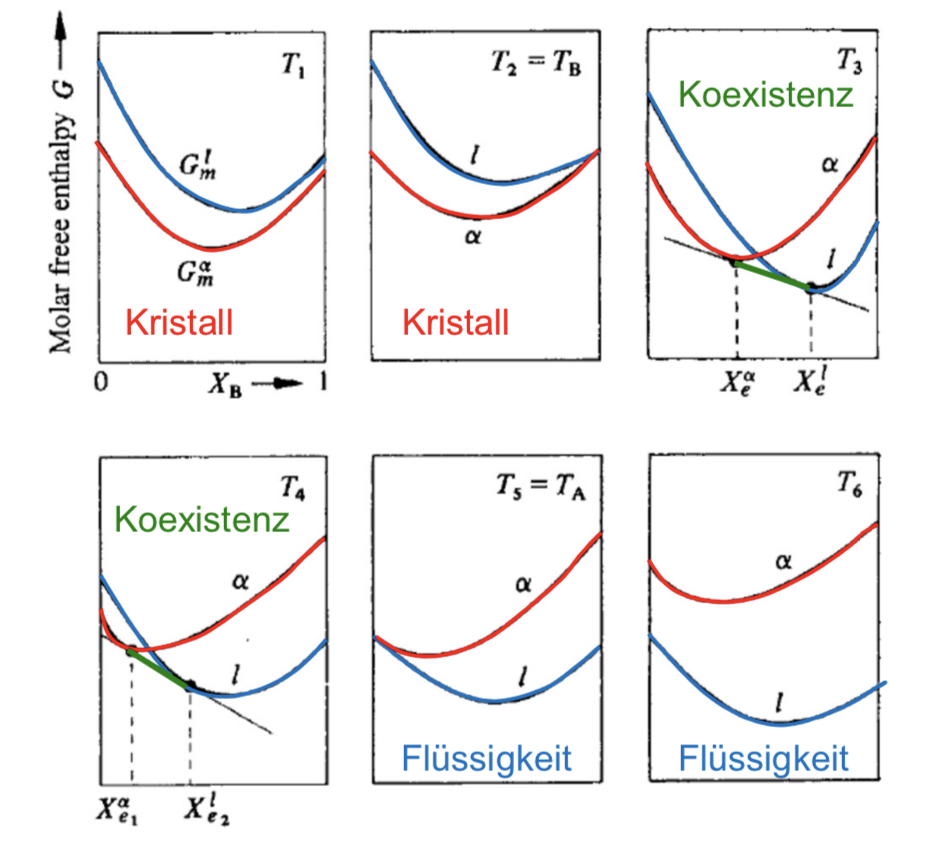
\includegraphics[width = 0.8\textwidth]{images/Materialwissenschaften/Mischungsenthalpie_Phasendiagramm.jpeg}
    \caption{Die freie Enthalpie in Abhängigkeit von der Zusammensetzung für verschiedene Temperaturen zur Bestimmung des Phasendiagramms.}
    \label{fig:Mischungsenthalpie_Phasendiagramm}
\end{figure}
\end{addmargin}

\end{document}